\documentclass[border=6pt]{standalone}
\usepackage{lmodern}
\usepackage[T1]{fontenc}
\usepackage{amsmath}
\usepackage{bm}
\usepackage{xcolor}
\usepackage{tikz}
\usetikzlibrary{arrows.meta,positioning}
\definecolor{cgray}{HTML}{6E6C66}
\definecolor{cblue}{HTML}{2F7DC8}
\definecolor{cgreen}{HTML}{4E8E2A}
\definecolor{cink}{HTML}{2B2B2B}
\tikzset{>={Stealth[length=2.2mm]}}
\newcommand{\fR}[1]{1.7*exp(0-((#1+0.85)*(#1+0.85))/1.0)}
\newcommand{\fE}[1]{1.7*exp(0-((#1-0.85)*(#1-0.85))/1.0)}
\begin{document}
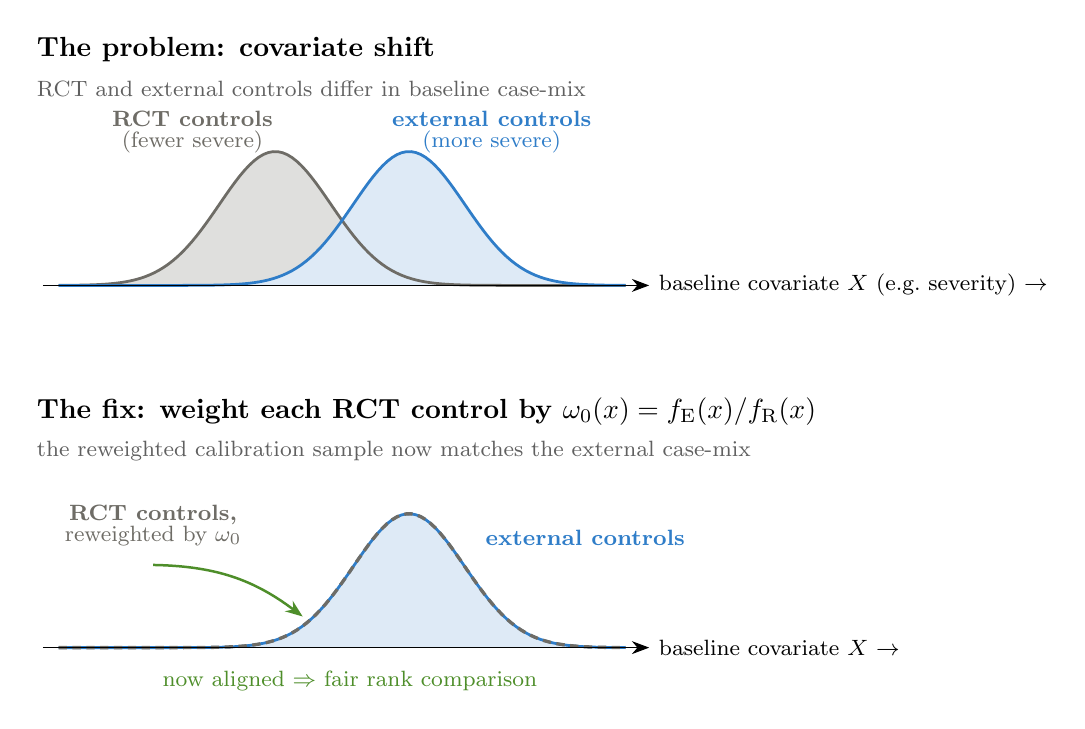
\begin{tikzpicture}[font=\small]

% ===== TOP: the problem =====
\begin{scope}
  \node[font=\bfseries,anchor=west] at (-4.0,3.0) {The problem: covariate shift};
  \node[font=\footnotesize,anchor=west,text=cink!75] at (-4.0,2.5) {RCT and external controls differ in baseline case-mix};
  \fill[cgray!22] (-3.6,0) -- plot[domain=-3.6:3.6,samples=90] (\x,{\fR{\x}}) -- (3.6,0) -- cycle;
  \fill[cblue!16] (-3.6,0) -- plot[domain=-3.6:3.6,samples=90] (\x,{\fE{\x}}) -- (3.6,0) -- cycle;
  \draw[cgray,line width=1.0pt] plot[domain=-3.6:3.6,samples=120] (\x,{\fR{\x}});
  \draw[cblue,line width=1.0pt] plot[domain=-3.6:3.6,samples=120] (\x,{\fE{\x}});
  \draw[->] (-3.8,0) -- (3.9,0) node[right,font=\footnotesize]{baseline covariate $X$ (e.g.\ severity) $\rightarrow$};
  \node[cgray,font=\footnotesize\bfseries,align=center] at (-1.9,1.95) {RCT controls\\[-2pt]\mdseries(fewer severe)};
  \node[cblue,font=\footnotesize\bfseries,align=center] at (1.9,1.95) {external controls\\[-2pt]\mdseries(more severe)};
\end{scope}

% ===== BOTTOM: the fix =====
\begin{scope}[yshift=-4.6cm]
  \node[font=\bfseries,anchor=west] at (-4.0,3.0) {The fix: weight each RCT control by $\omega_0(x)=f_{\mathrm E}(x)/f_{\mathrm R}(x)$};
  \node[font=\footnotesize,anchor=west,text=cink!75] at (-4.0,2.5) {the reweighted calibration sample now matches the external case-mix};
  \fill[cblue!16] (-3.6,0) -- plot[domain=-3.6:3.6,samples=90] (\x,{\fE{\x}}) -- (3.6,0) -- cycle;
  \draw[cblue,line width=1.0pt] plot[domain=-3.6:3.6,samples=120] (\x,{\fE{\x}});
  \draw[cgray,line width=1.2pt,densely dashed] plot[domain=-3.6:3.6,samples=120] (\x,{\fE{\x}});
  \draw[->] (-3.8,0) -- (3.9,0) node[right,font=\footnotesize]{baseline covariate $X$ $\rightarrow$};
  \node[cgray,font=\footnotesize\bfseries,align=center] at (-2.4,1.55) {RCT controls,\\[-2pt]\mdseries reweighted by $\omega_0$};
  \node[cblue,font=\footnotesize\bfseries,anchor=west] at (1.7,1.4) {external controls};
  \draw[->,cgreen,line width=0.9pt] (-2.4,1.05) to[bend left=18] (-0.5,{\fE{-0.5}+0.12});
  \node[cgreen,font=\footnotesize,anchor=north] at (0.1,-0.18) {now aligned $\Rightarrow$ fair rank comparison};
\end{scope}

\end{tikzpicture}
\end{document}
